\documentclass{article}
\usepackage{setspace,tikz}
\usepackage[text={6.5in,8.5in},centering]{geometry}
\geometry{verbose,a4paper,tmargin=2.4cm,bmargin=2.4cm,lmargin=2.4cm,rmargin=2.4cm}
\usepackage{graphicx,amsmath,cases,multirow,appendix,graphicx,xcolor}

\setlength\parindent{0pt}

\newcommand{\note}[1]{\colorbox{gray!20}{#1}}
\newcommand*\circled[1]{\tikz[baseline=(char.base)]{
            \node[shape=circle,draw,inner sep=2pt] (char) {#1};}}

\begin{document}


\noindent\makebox[\textwidth][c]{\Large\bfseries Lecture 2 - Summary}

Purpose of last lecture was to show connections between model equations that most of you have probably seen before:

\begin{center}
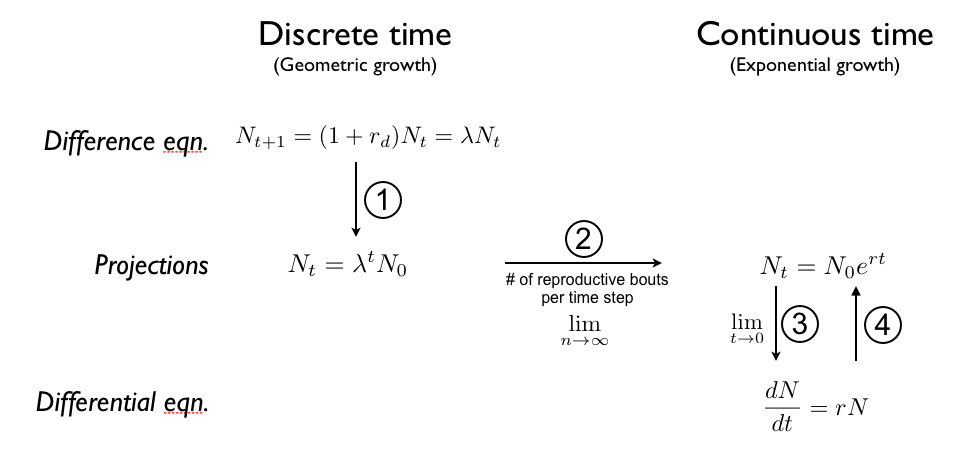
\includegraphics[width=16cm]{figs/EqnConnections.png}
\end{center}

\rule[0.5ex]{\linewidth}{1pt}

\circled{1}
e.g.,
\begin{equation*}
	N_{t+2}=\lambda N_{t+1}= \lambda (\underbrace{\lambda N_t}_{N_{t+1}}) = \lambda^2 N_t
\end{equation*}


\rule[0.5ex]{\linewidth}{1pt}

\circled{2}
Demonstration of how Euler's number $e$ emerges:
\begin{equation*}
	\boxed{ \lim_{n \to \infty}\left(1+\tfrac{1}{n}\right)^n	= e^1=e}
\end{equation*}
Let $r_d=1;  \;\; t=1 \; year$
\begin{align*}
\text{1 event per time-step:}&\\
	& N_1 = \lambda N_0=(1+r_d)N_0\\[1.5em]
\text{2 events per time-step:}&\\
	& N_1 = \lambda^2 N_0 = \left(1+\tfrac{r_d}{2}\right)^2 N_0 \\[1.5em]
n \text{ events per time-step:}&\\
	& N_1 = \left(1+\tfrac{r_d}{n}\right)^n N_0\\
	 \lambda  = & \frac{N_1}{N_0}=\left(1+\tfrac{r_d}{n}\right)^n\\
\text{Limit as }n \text{ goes to infinitity:}&\\
	\lambda = & \lim_{n \to \infty}\left(1+\tfrac{r_d}{n}\right)^n = e^r \\[1em]
\end{align*}
Therefore:
\begin{equation*}
	\lambda = (1+r_d) = e^r
\end{equation*}
And we have:
\begin{equation*}
	N_t=N_0 \lambda^t=  N_0 e^{rt}
\end{equation*}

\rule[0.5ex]{\linewidth}{1pt}
\pagebreak

\rule[0.5ex]{\linewidth}{1pt}

Defining the natural-log as the `anti-exponential' --- $ln(e^x)=x$ --- we also have:
\begin{equation*}
	ln(\lambda)=ln(1+r_d)=r
\end{equation*}
All three reflect the \emph{intrinsic per capita growth rate}:
\begin{align*}
	r_d= & b_d-d_d &\text{discrete time}\\
	r=& b-d & \text{continuous time}
\end{align*}

\rule[0.5ex]{\linewidth}{1pt}

\circled{3}  How to we get instantaneous population-level growth rate from projection equation, $N_0 e^{rt}$?\\ That is, how do we show that:
\begin{equation*}
\lim_{\Delta t \to 0}\left(\frac{\Delta N_t}{\Delta t}\right) = \frac{dN}{dt}
\end{equation*}

Need to take the derivative of $N_0 e^{rt}$ with respect to time $t$.

Use Chain Rule:
\begin{equation*}
\frac{d(XY)}{dt}=\frac{d(X)}{dt}\cdot Y + X \cdot \frac{d(Y)}{dt}
\end{equation*}
(The derivative of a product is the sum of the product of the derivative of each term times the other term.)
Thus:
\begin{equation*}
\frac{d(N_0 \cdot e^{rt})}{dt}=\frac{d(N_0)}{dt}\cdot (e^r)^t + N_0 \cdot \frac{d((e^r)^t)}{dt}
\end{equation*}

Note:\\
Derivative of a constant = 0\\
Derivative of $a^x = ln(a)\cdot a^x$.

Thus:
\begin{align*}
	\frac{d(N_0 e ^{rt})}{dt} & =0 \cdot (e^r)^t + ln(e^r)\cdot (e^r)^t \cdot N_0\\
	&= r \cdot (e^r)^t \cdot N_0\\
	&= r \cdot e^{rt} \cdot N_0 \\
	&= r \cdot N_0 e^{rt} \\
\text{Since } N=N_0 e^{rt} \text{ for any time } t ...&\\
	&=rN=\frac{dN}{dt}
\end{align*}


\rule[0.5ex]{\linewidth}{1pt}

\circled{4} Could also go in opposite direction from $\frac{dN}{dt} \rightarrow N_0 e^{rt}$:
\begin{align*}
&	\frac{dN}{dt}=rN\\
&	\frac{1}{N}\frac{dN}{dt}=r\\
&	\int_0^T \frac{1}{N}\frac{dN}{dt} \; dt = \int_0^T r\; dt \;\;\;\;(\text{Think of T as a constant, and t in dt as a variable})\\
&	\int_0^T \frac{1}{N}\frac{dN}{dt}  = r t \vert_0^T = r \cdot T - r \cdot 0\\
	\text{Using} \; \int \frac{1}{x}\; dx = ln(x)...\\
&	ln(N(T))-ln(N(0))=rT\\
& ln\left( \frac{N(T)}{N(0)}\right) = rT\\
& \frac{N(T)}{N(0)}= e^{rT}\\
& N(T)=N(0)e^{rT}
\end{align*}


\rule[0.5ex]{\linewidth}{1pt}

\end{document}